% !TEX program = xelatex
% 第一讲：examples.tex + equations.tex
\documentclass[fontset=windows, chinese, 10pt, xcolor=dvipsnames]{beamer}
% Shared preamble for the chapter 05 standalone lectures.
% Each lecture sets \title and \subtitle after this file is read.

\usepackage{amsmath,amssymb,mathtools}
\usepackage{xeCJK}
\usepackage{zhnumber}
\usepackage{tikz}
\usetikzlibrary{arrows.meta,calc,positioning}

\usetheme{metropolis}
\usepackage{beamercolorthemeHistNanjing}

\newcommand{\red}[1]{\textcolor{red}{#1}}
\newcommand{\blue}[1]{\textcolor{blue}{#1}}
\newcommand{\green}[1]{\textcolor{green}{#1}}
\newcommand{\gray}[1]{\textcolor{gray}{#1}}
\newcommand{\orange}[1]{\textcolor{orange}{#1}}

\newcommand{\sssub}[1]{ {\mathrm{#1} }}  % script size subscript\\\
\newcommand{\funcd}[2]{ \frac{d{#1}}{d{#2}}} %function full derivative
\newcommand{\funcpd}[2]{ \frac{\partial{#1}}{\partial{#2}}} %function partial derivative
\newcommand{\fnald}[2] { \frac{\delta {#1}}{\delta {#2}}} % functional derivative

\renewcommand{\Re}{\operatorname{Re}}
\renewcommand{\Im}{\operatorname{Im}}
\def\ext{\sssub{ext}}
\def\x{\sssub{x}}
\def\xc{\sssub{xc}}
\def\H{\sssub{H}}
\def\Hx{\sssub{Hx}}
\def\Hxc{\sssub{Hxc}}
\def\c{\sssub{c}}
\def\s{\sssub{s}}

% \def\ext{\sssub{ext}}
% \def\ext{\sssub{ext}}
% \def\ext{\sssub{ext}}
% \def\ext{\sssub{ext}}
% \defsssub{ext}


% definitions of bold faced symbols
\def\brpppp{{\mathbf{r}^{\prime\prime\prime\prime}}}
\def\brppp{{\mathbf{r}^{\prime\prime\prime}}}
\def\brpp{{\mathbf{r}^{\prime\prime}}}
\def\brp{{\mathbf{r}^{\prime}}}
\def\bzp{{\mathbf{z}^{\prime}}}
\def\bxp{{\mathbf{x}^{\prime}}}
\def\tp{{{t}^{\prime}}}
\def\tpp{{{t}^{\prime\prime}}}
\def\tppp{{{t}^{\prime\prime\prime}}}

\def\tbr{{\tilde{\mathbf{r}}}}
\def\bk{{\mathbf{k}}}
\def\br{{\mathbf{r}}}
\def\bp{{\mathbf{p}}}
\def\bq{{\mathbf{q}}}
\def\bv{{\mathbf{v}}}
\def\bz{{\mathbf{z}}}
\def\mbf{{\mathbf{f}}}

\def\bx{{\mathbf{x}}}
\def\bR{{\mathbf{R}}}
\def\bM{{\mathbf{M}}}
\def\bP{{\mathbf{P}}}
\def\bT{{\mathbf{T}}}
\def\bK{{\mathbf{K}}}
\def\bA{{\mathbf{A}}}
\def\bB{{\mathbf{B}}}
\def\bD{{\mathbf{D}}}
\def\bE{{\mathbf{E}}}
\def\bF{{\mathbf{F}}}
\def\bG{{\mathbf{G}}}
\def\bH{{\mathbf{H}}}
\def\bI{{\mathbf{I}}}
\def\bJ{{\mathbf{J}}}
\def\bP{{\mathbf{P}}}
\def\bS{{\mathbf{S}}}
\def\bV{{\mathbf{V}}}
\def\bX{{\mathbf{X}}}
\def\bY{{\mathbf{Y}}}
\def\dd{{\mathop{}\!\mathrm{d}}}
\def\dr{{\!\!\dd\br\,}}
\def\dx{{\!\!\dd\bx\,}}
\def\dy{{\!\!\dd\by\,}}
\def\dk{{\!\!\dd\bk\,}}
\def\dG{{\!\!\dd\bG\,}}


\def\half{{\frac{1}{2}}}
\def\tr{{\mathrm{tr}}}


\def\Arg{{\mathrm{Arg}\;}}
\def\arg{{\mathrm{arg}\;}}
\def\Res{{\mathrm{Res}\;}}


\author{罗凯}
\institute{南京理工大学物理学院}
\date{\zhdigits{\the\year},\zhganzhinian{\the\year}年秋}

\usebackgroundtemplate{%
\begin{tikzpicture}[remember picture,overlay]
  \node[opacity=0.05, at=(current page.center)] {
    
\includegraphics[width=0.6\paperwidth]{njust-logo.jpeg}
  };
\end{tikzpicture}}


\title{数学物理方程}
\subtitle{第一讲：典型方程及其物理来源}

\begin{document}

\begin{frame}
  \titlepage
\end{frame}

\begin{frame}{本章从哪里开始}
  \begin{quote}
    致知在格物。\\
    \hfill ——《大学》
  \end{quote}
  格物，是认真观察现象，并追问支配它们的道理。
  数学物理沿这条路走：把观测、对称性和守恒定律写成方程。
  \vspace{0.4em}

  本章要做三件事：推出波动、扩散和势的标准方程；说明怎样的数据才能定出一个物理的解；再用分离变量处理典型的边值问题。
\end{frame}

\begin{frame}{三讲安排}
  \begin{enumerate}
    \item \textbf{本讲}：偏微分方程的例子，以及弦振动、热传导、拉普拉斯与泊松方程的推导。
    \item 第二讲：初始条件、边界条件、稳态问题，以及二阶方程的分类与标准形。
    \item 第三讲：分离变量法。两端固定的弦，以及均匀电场中的长直圆柱。
  \end{enumerate}
  \vspace{0.6em}
  同一条方程可以出现在很不一样的场合；同一类现象，换一组物理假定，也会得到不同的方程。
\end{frame}

\begin{frame}{本讲要回答的三个问题}
  \begin{enumerate}
    \item 琴弦被拨动以后，位移 $u(x,t)$ 怎样运动？
    \item 一根细杆两端维持不同温度，杆内的温度怎样变化，又怎样达到稳定？
    \item 两块导体板之间没有电荷时，电势和电场是什么样子？
  \end{enumerate}
  \vspace{0.5em}
  三条问题分别引出波动、热传导和拉普拉斯方程。先弄清什么叫“解”，再从平衡律把方程推出来，每推完一条就代一个具体的函数检验。更广的方程目录放在最后，用来辨认它们像这三条中的哪一条。
\end{frame}

% =============================================================
\section{方程举例}

\subsection{什么是偏微分方程}

\begin{frame}{偏微分方程}
  \textbf{偏微分方程}（partial differential equation, PDE）把多个自变量的未知函数和它的偏导数联系起来。
  \begin{itemize}
    \item 自变量常常是位置 $\mathbf{x}$ 和时间 $t$，也可以是动量或参数。
    \item 未知量可以是一个标量场 $u$，也可以是向量场或张量场。
    \item 不含时间的方程称为\textbf{稳态}方程；含时间导数的方程描述\textbf{演化}。
  \end{itemize}
  “解”不是一个数，而是一个函数：把它代进方程，方程变成恒等式。下面用输运方程把这件事做一遍。
\end{frame}

\subsection{输运与守恒}

\begin{frame}{一阶输运方程}
  一阶输运方程
  \begin{equation*}
    u_t+c\,u_x=0
  \end{equation*}
  描述以常速 $c$ 传播、形状不变的剖面。它的解是
  \begin{equation*}
    u(x,t)=g(x-ct).
  \end{equation*}
  把 $g(\xi)$ 代入即得 $u_t=-cg'$，$u_x=g'$，两者相加为零。
  \vspace{0.3em}

  它可以表示一维均匀流动所携带的示踪物浓度：波形整体平移，不摊平，也不来回振荡。
\end{frame}

\begin{frame}{例：一个鼓包在移动}
  取 $c=2$，初始鼓包 $g(\xi)=e^{-\xi^2}$。则
  \begin{equation*}
    u(x,t)=e^{-(x-2t)^2}.
  \end{equation*}
  \begin{columns}[c]
    \begin{column}{0.48\textwidth}
      \begin{itemize}
        \item $t=0$ 时峰在 $x=0$。
        \item $t=1$ 时峰在 $x=2$，$t=3$ 时峰在 $x=6$。
        \item 高度和宽度都不变。
      \end{itemize}
      若误写成 $e^{-(x+2t)^2}$，峰向左跑，满足的是 $u_t-2u_x=0$，不是原方程。符号决定方向。
    \end{column}
    \begin{column}{0.48\textwidth}
      \centering
      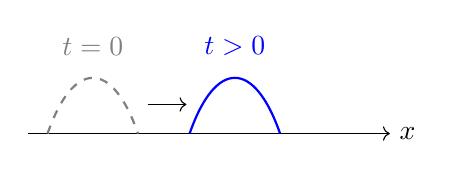
\begin{tikzpicture}[scale=0.82]
        \draw[->] (0,0) -- (5.6,0) node[right] {$x$};
        \draw[gray,dashed,thick] (0.3,0)
          .. controls (0.7,1.15) and (1.3,1.15) .. (1.7,0);
        \draw[blue,thick] (2.5,0)
          .. controls (2.9,1.15) and (3.5,1.15) .. (3.9,0);
        \node[gray] at (1.0,1.35) {$t=0$};
        \node[blue] at (3.2,1.35) {$t>0$};
        \draw[->] (1.85,0.45) -- (2.45,0.45);
      \end{tikzpicture}
    \end{column}
  \end{columns}
\end{frame}

\begin{frame}{连续性方程}
  更一般地，守恒密度 $\rho(\mathbf{x},t)$ 与通量 $\mathbf{J}$ 满足\textbf{连续性方程}
  \begin{equation*}
    \rho_t+\nabla\cdot\mathbf{J}=s,
  \end{equation*}
  其中 $s$ 是源或汇。对速度为 $\mathbf{v}$ 的流体，$\mathbf{J}=\rho\mathbf{v}$，质量守恒写成
  \begin{equation*}
    \rho_t+\nabla\cdot(\rho\mathbf{v})=0.
  \end{equation*}
  散度项量度小体积上的净流出。热传导和电荷守恒也是同一种平衡律，只是通量由不同的本构关系给出。弦的推导就是对横向动量写这条平衡。
\end{frame}

\begin{frame}{从这里进入推导}
  输运方程的通量是 $c u$，事先给定。弦和热传导不同：通量或力由未知函数自己的斜率决定，平衡律因此含有二阶导数。
  \vspace{0.5em}

  顺序是：弦的动量平衡，热的能量平衡，再令时间导数为零得到稳态。每条方程推出后，立刻代一个显式的函数，确认它确实是解。
\end{frame}

% The wider catalogue is postponed until the three equations can be recognized.
% =============================================================
\section{弦振动方程}

\subsection{模型与小段受力}

\begin{frame}{弦的物理图像}
  弦振动方程在十八世纪由达朗贝尔等人系统研究，是一大类偏微分方程的原型。
  \vspace{0.3em}

  考虑长为 $\ell$、两端固定、张紧的均匀柔软弦，求它在平衡位置附近的小横振动。
  \begin{center}
  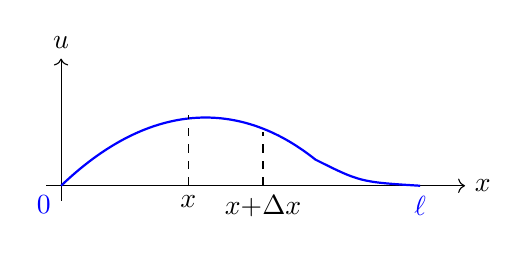
\begin{tikzpicture}[scale=0.95]
    \draw[->] (-0.2,0) -- (5.4,0) node[right] {$x$};
    \draw[->] (0,-0.2) -- (0,1.7) node[above] {$u$};
    \draw[thick,blue] (0,0) node[below left] {$0$}
      .. controls (1.2,1.15) and (2.4,1.15) .. (3.4,0.35)
      .. controls (4.0,0.05) .. (4.8,0) node[below] {$\ell$};
    \draw[dashed] (1.7,0) -- (1.7,0.95);
    \draw[dashed] (2.7,0) -- (2.7,0.72);
    \node[below] at (1.7,0) {$x$};
    \node[below] at (2.7,0) {$x{+}\Delta x$};
  \end{tikzpicture}
  \end{center}
  固定时刻 $t$ 的图像 $u(x,t)$ 就是弦在该时刻的形状。
\end{frame}

\begin{frame}{三条理想化}
  把物理问题写成数学模型时，保留主导效应：
  \begin{enumerate}
    \item 弦是均匀的，直径远小于长度，可用线密度为常数 $\rho$ 的曲线表示。
    \item 运动限制在一个平面内，并且是横向的：每个质点垂直于平衡的 $x$ 轴作小位移。
    \item 弦完全柔软，不抵抗弯曲。张力沿变形后的弦的切向，伸长服从胡克定律。
  \end{enumerate}
  先不考虑外力。端点放在 $x=0$ 和 $x=\ell$。
\end{frame}

\begin{frame}{小段的弧长}
  取 $x$ 到 $x+\Delta x$ 的一小段，弧长为
  \begin{equation*}
    \Delta s=\int_x^{x+\Delta x}\sqrt{1+u_x(\xi,t)^2}\,\mathrm{d}\xi.
  \end{equation*}
  振动很小，$u_x^2$ 相对 $1$ 可以忽略，于是 $\Delta s\approx\Delta x$。
  \vspace{0.4em}

  这一小段几乎没有额外伸长。张力因此不随时间变化；下面的水平力平衡还会说明，它的大小也不随 $x$ 变化。
\end{frame}

\begin{frame}{张力的分量}
  设左端张力大小为 $T(x)$，$\alpha_1,\alpha_2$ 分别是 $x$ 与 $x+\Delta x$ 处切线和 $x$ 轴的夹角。作用在小段上的张力分量为
  \begin{equation*}
    \begin{array}{c|cc}
      & x\text{ 分量} & u\text{ 分量}\\ \hline
      x & -T(x)\cos\alpha_1 & -T(x)\sin\alpha_1\\
      x+\Delta x & T(x+\Delta x)\cos\alpha_2 & T(x+\Delta x)\sin\alpha_2.
    \end{array}
  \end{equation*}
  水平方向没有加速度，所以水平合力为零。
\end{frame}

\begin{frame}{小斜率：张力为常数}
  小振动时
  \begin{equation*}
    \cos\alpha_1=\frac{1}{\sqrt{1+u_x(x,t)^2}}\approx 1,
    \qquad \cos\alpha_2\approx 1,
  \end{equation*}
  水平平衡给出 $T(x+\Delta x)=T(x)=T$。同样，
  \begin{equation*}
    \sin\alpha_1\approx\tan\alpha_1=u_x(x,t),
    \qquad
    \sin\alpha_2\approx u_x(x+\Delta x,t).
  \end{equation*}
  净横向力因此是
  \begin{equation*}
    T\bigl[u_x(x+\Delta x,t)-u_x(x,t)\bigr].
  \end{equation*}
\end{frame}

\subsection{从冲量到波动方程}

\begin{frame}{冲量写成二重积分}
  在短时间 $[t,t+\Delta t]$ 上使用冲量--动量定理。张力的冲量为
  \begin{equation*}
    \int_t^{t+\Delta t}
      T\bigl[u_x(x+\Delta x,\tau)-u_x(x,\tau)\bigr]\,\mathrm{d}\tau.
  \end{equation*}
  对 $x$ 用牛顿--莱布尼茨公式，$u_x(x+\Delta x)-u_x(x)=\int_x^{x+\Delta x}u_{xx}\,\mathrm{d}\xi$，故冲量等于
  \begin{equation*}
    \int_t^{t+\Delta t}\int_x^{x+\Delta x} T u_{xx}(\xi,\tau)\,\mathrm{d}\xi\,\mathrm{d}\tau.
  \end{equation*}
\end{frame}

\begin{frame}{动量变化}
  小段的横向动量是 $\displaystyle\int_x^{x+\Delta x}\rho u_t(\xi,t)\,\mathrm{d}\xi$。它在 $\Delta t$ 内的变化为
  \begin{equation*}
    \int_x^{x+\Delta x}\rho\bigl[u_t(\xi,t+\Delta t)-u_t(\xi,t)\bigr]\,\mathrm{d}\xi
    =\int_t^{t+\Delta t}\int_x^{x+\Delta x}\rho u_{tt}\,\mathrm{d}\xi\,\mathrm{d}\tau.
  \end{equation*}
  冲量等于动量变化，移项后
  \begin{equation*}
    \int_t^{t+\Delta t}\int_x^{x+\Delta x}
      \bigl(T u_{xx}-\rho u_{tt}\bigr)\,\mathrm{d}\xi\,\mathrm{d}\tau=0.
  \end{equation*}
\end{frame}

\begin{frame}{自由振动方程}
  空间间隔和时间间隔都是任意的。被积函数连续时，积分在每个小矩形上都为零，只能是被积函数本身为零：
  \begin{equation*}
    \rho u_{tt}=T u_{xx}.
  \end{equation*}
  记 $a^2=T/\rho$，得到自由振动方程
  \begin{equation*}
    \boxed{u_{tt}-a^2 u_{xx}=0.}
  \end{equation*}
  $a=\sqrt{T/\rho}$ 是波速。张力越大、弦越轻，波跑得越快。
\end{frame}

\begin{frame}{例：右行波是解}
  在整条直线上设 $u(x,t)=g(x-at)$，记 $\xi=x-at$。则
  \begin{align*}
    u_t&=-a g'(\xi), & u_{tt}&=a^2 g''(\xi),\\
    u_x&=g'(\xi), & u_{xx}&=g''(\xi).
  \end{align*}
  因此 $u_{tt}-a^2 u_{xx}=0$。$g(x+at)$ 是左行波，同样是解。
  \vspace{0.4em}

  固定端点还没放进来。$g(x-at)$ 一般不能在 $x=0$ 和 $x=\ell$ 同时为零，所以它还不是两端固定那根弦的运动。方程的解很多，边界把它们挑掉一批。这是第二讲的起点。
\end{frame}

\begin{frame}{例：波速的一个数字}
  线密度 $\rho=0.01\,\mathrm{kg/m}$，张力 $T=100\,\mathrm{N}$。
  \begin{equation*}
    a=\sqrt{T/\rho}=\sqrt{100/0.01}=100\,\mathrm{m/s}.
  \end{equation*}
  右行鼓包的峰若在 $t=0$ 时位于 $x=0.2\,\mathrm{m}$，则在 $t=0.01\,\mathrm{s}$ 时位于
  \begin{equation*}
    x=0.2+at=0.2+1=1.2\,\mathrm{m}.
  \end{equation*}
  把张力提高四倍，$a$ 只提高两倍。波速看的是 $T/\rho$ 的平方根，不是张力本身。
\end{frame}

\begin{frame}{这个方程用在哪里}
  推导只用了：均匀、柔软、张紧，以及小横向振动。
  \begin{itemize}
    \item 振幅很大时，$u_x^2$ 不能丢掉，张力也不再是常数，方程变成非线性的。
    \item 弦若抵抗弯曲，恢复力不再只来自张力的横向分量，方程里会出现 $u_{xxxx}$。本讲末尾的梁方程就是这种模型。
  \end{itemize}
  模型的用处和限度都由这些假定决定。
\end{frame}

\begin{frame}{外力与受迫振动}
  设横向外力密度为 $F(x,t)$。它在 $[t,t+\Delta t]$ 内对小段的冲量是
  \begin{equation*}
    \int_t^{t+\Delta t}\int_x^{x+\Delta x} F(\xi,\tau)\,\mathrm{d}\xi\,\mathrm{d}\tau.
  \end{equation*}
  加到前面的平衡里，
  \begin{equation*}
    \int_t^{t+\Delta t}\int_x^{x+\Delta x}
      \bigl(T u_{xx}-\rho u_{tt}+F\bigr)\,\mathrm{d}\xi\,\mathrm{d}\tau=0.
  \end{equation*}
  再由区间的任意性，并令 $f=F/\rho$，得到
  \begin{equation*}
    \boxed{u_{tt}-a^2 u_{xx}=f(x,t),\qquad f=\dfrac{F}{\rho}.}
  \end{equation*}
  变化以有限速度 $a$ 传播。只知道方程、不知道弦在 $t=0$ 的位置和速度，运动还不能确定。
\end{frame}

% =============================================================
\section{热传导方程}

\subsection{傅里叶定律与能量平衡}

\begin{frame}{傅里叶定律}
  设物体 $G$ 在位置 $(x,y,z)$、时刻 $t$ 的温度为 $u(x,y,z,t)$。热流与温度的局部关系是傅里叶实验定律：在 $\mathrm{d}t$ 内，沿外法向 $\mathbf{n}$ 穿过有向面元 $\mathrm{d}S$ 的热量为
  \begin{equation*}
    \mathrm{d}Q=-k(x,y,z)\frac{\partial u}{\partial n}\,\mathrm{d}S\,\mathrm{d}t.
  \end{equation*}
  $k>0$ 是热传导系数。负号是实质内容：\textbf{热从高温流向低温}，与 $u$ 增加的方向相反。
\end{frame}

\begin{frame}{流入的热量}
  在物体内部任取闭曲面 $\Gamma$，它围出区域 $\Omega$。从 $t_1$ 到 $t_2$ \emph{流入} $\Omega$ 的热量为
  \begin{equation*}
    Q=\int_{t_1}^{t_2}\iint_{\Gamma} k\frac{\partial u}{\partial n}\,\mathrm{d}S\,\mathrm{d}t.
  \end{equation*}
  符号相对傅里叶定律反了一次：$\partial u/\partial n$ 用的是外法向，而正的 $Q$ 定义为进入区域的热。
\end{frame}

\begin{frame}{内能的增加}
  设比热为 $c(x,y,z)$，质量密度为 $\rho(x,y,z)$。同一时间间隔内，内能的增加是
  \begin{equation*}
    \iiint_{\Omega}\rho c\,
      \bigl[u(x,y,z,t_2)-u(x,y,z,t_1)\bigr]\,\mathrm{d}V.
  \end{equation*}
  能量守恒要求它等于流入的热量 $Q$。假定 $u$ 的二阶空间导数和一阶时间导数都连续。
\end{frame}

\begin{frame}{散度定理}
  散度定理把曲面积分改成体积分：
  \begin{equation*}
    \int_{t_1}^{t_2}\iiint_{\Omega}\nabla\cdot(k\nabla u)\,\mathrm{d}V\,\mathrm{d}t
    =\iiint_{\Omega}\rho c\left(\int_{t_1}^{t_2}u_t\,\mathrm{d}t\right)\mathrm{d}V.
  \end{equation*}
  交换积分次序，得到
  \begin{equation*}
    \int_{t_1}^{t_2}\iiint_{\Omega}
      \bigl[\rho c\,u_t-\nabla\cdot(k\nabla u)\bigr]\,\mathrm{d}V\,\mathrm{d}t=0.
  \end{equation*}
\end{frame}

\begin{frame}{一般的热传导方程}
  时间间隔和区域 $\Omega$ 都是任意的，被积函数必须为零。非均匀各向同性物体的热传导方程是
  \begin{equation*}
    \boxed{\rho c\,u_t=\nabla\cdot(k\nabla u).}
  \end{equation*}
  若 $k$ 不是常数，右边不是 $k\nabla^2u$，而是
  \(\nabla\cdot(k\nabla u)=k\nabla^2u+\nabla k\cdot\nabla u\)。
  传导系数的空间变化本身会贡献一项。
\end{frame}

\begin{frame}{均匀介质}
  物体均匀时，$k,c,\rho$ 都是常数。令 $\kappa=k/(\rho c)$，
  \begin{equation*}
    \nabla^2=\partial_{xx}+\partial_{yy}+\partial_{zz},
  \end{equation*}
  方程化为齐次\textbf{热方程}
  \begin{equation*}
    \boxed{u_t=\kappa\nabla^2u.}
  \end{equation*}
  扩散把温差抹平，而不是把一个尖锐扰动以固定速度送出去。
\end{frame}

\begin{frame}{例：峰顶降温，谷底升温}
  先看一根细杆上的 $u_t=\kappa u_{xx}$，$\kappa>0$。
  \begin{itemize}
    \item 在温度的局部极大处，$u_{xx}<0$，于是 $u_t<0$：峰顶变凉。
    \item 在局部极小处，$u_{xx}>0$，于是 $u_t>0$：谷底变暖。
  \end{itemize}
  同一条曲率，在波动方程里作用不同。$u_{tt}=a^2 u_{xx}$ 在峰顶给出向下的加速度，弦冲过平衡位置，所以会振荡；热方程没有二阶时间导数，峰顶只是下降，不会冲到另一侧。
\end{frame}

\begin{frame}{有热源的情形}
  设热源在单位体积内的产热率为 $F(x,y,z,t)$。它在能量平衡中的贡献是
  \begin{equation*}
    \int_{t_1}^{t_2}\iiint_{\Omega} F\,\mathrm{d}V\,\mathrm{d}t.
  \end{equation*}
  加进去以后，
  \begin{equation*}
    \rho c\,u_t=\nabla\cdot(k\nabla u)+F.
  \end{equation*}
  均匀介质中就是非齐次热方程
  \begin{equation*}
    \boxed{u_t=\kappa\nabla^2u+f,\qquad f=\frac{F}{\rho c}.}
  \end{equation*}
\end{frame}

% =============================================================
\section{拉普拉斯方程与泊松方程}

\subsection{从演化到平衡}

\begin{frame}{稳态留下椭圆型方程}
  许多系统演化到力、通量或源彼此平衡为止。稳态下时间导数消失，留下椭圆型方程。三维中两个中心的稳态场方程是
  \begin{equation*}
    \boxed{\nabla^2u=0}
    \qquad\text{与}\qquad
    \boxed{\nabla^2u=f.}
  \end{equation*}
  第一个是\textbf{拉普拉斯方程}，它的解称为\textbf{调和函数}。第二个是\textbf{泊松方程}，$f$ 表示源。
  直角坐标中 $\nabla^2u=u_{xx}+u_{yy}+u_{zz}$。
\end{frame}

\begin{frame}{源项的符号}
  $f$ 的符号和物理含义依赖所选的模型。结构上的区别是：
  \begin{itemize}
    \item 无源区域用拉普拉斯方程；
    \item 有分布源时用泊松方程。
  \end{itemize}
  下面三个例子里，$f$ 分别是 $-F/T$、$-F/k$ 和 $-\rho_e/\varepsilon_0$。负号来自恢复力、傅里叶定律或电场的定义，不是拉普拉斯算子本身的约定。
\end{frame}

\subsection{膜与稳态热流}

\begin{frame}{薄膜的平衡}
  均匀张力为 $T$、面密度为 $\rho$ 的薄膜，横向位移 $u(x,y,t)$，横向力密度 $F(x,y,t)$。小振动方程是
  \begin{equation*}
    \rho u_{tt}=T(u_{xx}+u_{yy})+F.
  \end{equation*}
  这是二维的受迫波动方程，推导与弦相同：张力的净横向分量给出 $T\nabla^2u$。
  \vspace{0.4em}

  外力不随时间变化，膜又已经到达平衡，$u_{tt}=0$，形状满足
  \begin{equation*}
    u_{xx}+u_{yy}=-\frac{F(x,y)}{T}.
  \end{equation*}
  这是二维泊松方程。没有横向载荷时，平衡膜满足拉普拉斯方程。
\end{frame}

\begin{frame}{稳态温度}
  同一划分也来自热传导。稳态时 $u_t=0$。均匀材料、内部有稳定热源 $F$ 时，
  \begin{equation*}
    \nabla^2u=-\frac{F}{k}.
  \end{equation*}
  内部不产热时，稳态温度是调和函数。
  \vspace{0.4em}

  因此同一组数学方程既描述平衡形状，也描述平衡温度。物理不同，平衡条件的数学形式相同。
\end{frame}

\begin{frame}{例：均匀加热的平板}
  平板占据 $0\leq x\leq L$，热传导系数为常数，单位体积产热率 $F>0$ 为常数。两面温度保持为零：
  \begin{equation*}
    u''(x)=-\frac{F}{k},
    \qquad u(0)=u(L)=0.
  \end{equation*}
  积分一次，$u'=-(F/k)x+A$；再积分，
  \begin{equation*}
    u(x)=-\frac{F}{2k}x^2+Ax+B.
  \end{equation*}
\end{frame}

\begin{frame}{例：均匀加热的平板（定常数）}
  $u(0)=0$ 给出 $B=0$。$u(L)=0$ 给出
  \begin{equation*}
    A=\frac{F}{2k}L,
    \qquad
    \boxed{u(x)=\dfrac{F}{2k}\,x(L-x).}
  \end{equation*}
  这是开口向下的抛物线，最大值在板的中心 $x=L/2$，最大值为 $FL^2/(8k)$。
  中心处 $u''=-F/k<0$，和“峰顶曲率为负”一致。
  \vspace{0.3em}

  热在内部各处产生，再由传导送到较冷的边界。没有源时，同样的两端为零只允许 $u\equiv 0$：没有热可送。
\end{frame}

\subsection{静电势}

\begin{frame}{高斯定理}
  静电场的电场线起于正电荷、止于负电荷，在静电场中不形成闭圈。国际单位制下，对包围体积 $\Omega$ 的任意闭曲面 $\Sigma$，
  \begin{equation*}
    \oint_{\Sigma}\mathbf{E}\cdot\mathrm{d}\mathbf{S}
    =\frac{1}{\varepsilon_0}\iiint_{\Omega}\rho_e\,\mathrm{d}V.
  \end{equation*}
  用散度定理，并利用 $\Omega$ 的任意性，得到局部形式。再加上静电场旋度为零：
  \begin{equation*}
    \nabla\cdot\mathbf{E}=\frac{\rho_e}{\varepsilon_0},
    \qquad \nabla\times\mathbf{E}=0.
  \end{equation*}
\end{frame}

\begin{frame}{用标量势代替向量场}
  旋度为零，线积分与路径无关，因此存在标量势 $V$，使
  \begin{equation*}
    \mathbf{E}=-\nabla V.
  \end{equation*}
  代入高斯定理，
  \begin{equation*}
    \boxed{\nabla^2 V=-\dfrac{\rho_e}{\varepsilon_0}.}
  \end{equation*}
  有电荷处 $V$ 满足泊松方程，无电荷处满足拉普拉斯方程。
  \vspace{0.3em}

  用标量势代替向量场往往是决定性的简化：知道 $V$ 之后，物理场由 $\mathbf{E}=-\nabla V$ 给出。
\end{frame}

\begin{frame}{例：两块平行导电板}
  两块大平行导电板之间没有电荷，势只依赖垂直于板面的坐标 $x$。设 $V(0)=0$，$V(d)=V_0$，拉普拉斯方程化为
  \begin{equation*}
    V''(x)=0.
  \end{equation*}
  因此 $V(x)=Ax+B$。由 $V(0)=0$ 得 $B=0$，由 $V(d)=V_0$ 得 $A=V_0/d$，
  \begin{equation*}
    \boxed{V(x)=\dfrac{V_0}{d}x,
    \qquad
    \mathbf{E}=-\dfrac{V_0}{d}\,\mathbf{e}_x.}
  \end{equation*}
  若 $V_0>0$，右板电势更高，电场指向 $-x$，从高电势指向低电势。负号来自 $\mathbf{E}=-\nabla V$，不是额外假定。
\end{frame}

\begin{frame}{平行板与加热板对照}
  电势线性变化，电场均匀。这是加热板问题的无源对应：
  \begin{itemize}
    \item 无源时，内部场由边界值单独决定，一维稳态解是直线；
    \item 有均匀源时，内部多一次积分，解是抛物线。
  \end{itemize}
  二维和三维里同样的原则仍在，但直线和抛物线要换成级数或格林函数。那是第三讲和后面格林函数一章的内容。
\end{frame}


\section{辨认同一类方程}

\begin{frame}{先辨认，再看新方程}
  三条方程已经从平衡律里推出来，并且各配了一个能代回去的解。
  后面的例子不再推导。读每条方程时只问：
  \begin{enumerate}
    \item 它把一个剖面\textbf{原样送走}，还是\textbf{抹平}，还是描述\textbf{平衡}？
    \item 未知量是一个标量，还是向量、张量或一组联立的量？
    \item 最高阶导数是几阶？弦是二阶；梁和板因为抵抗弯曲，升到四阶。
  \end{enumerate}
\end{frame}

\begin{frame}{标量波动方程}
  $d$ 维空间中的标量\textbf{波动方程}是
  \begin{equation*}
    u_{tt}-c^2\nabla^2u=0.
  \end{equation*}
  它描述以速度 $c$ 传播的小扰动，包括均匀介质中的声波，以及弹性运动中适合用标量描述的部分。
  \vspace{0.4em}

  一维形式就是前面推出的弦振动方程，波速 $c=a=\sqrt{T/\rho}$。多出来的空间维数不改变“以有限速度传播”这件事。
\end{frame}

\begin{frame}{均匀各向同性弹性体}
  位移 $\mathbf{u}(\mathbf{x},t)$ 是向量。线性化模型为
  \begin{equation*}
    \rho\mathbf{u}_{tt}
    =(\lambda+\mu)\nabla(\nabla\cdot\mathbf{u})+\mu\nabla^2\mathbf{u},
  \end{equation*}
  其中 $\lambda,\mu$ 是拉梅参数。
  \begin{itemize}
    \item $\nabla\cdot\mathbf{u}$ 描述体积变化，对应压缩波。
    \item 其余部分描述形状变化，对应剪切波。
  \end{itemize}
  两种变形模式的传播速度不同，所以弹性波一般不能收成一个标量波动方程。
\end{frame}

\begin{frame}{梁与薄板：四阶导数}
  弯曲需要更高阶的空间导数。理想细梁可以满足
  \begin{equation*}
    u_{tt}+K u_{xxxx}=0,
  \end{equation*}
  理想薄板可以满足
  \begin{equation*}
    u_{tt}+K\nabla^4u=0,
    \qquad \nabla^4=(\nabla^2)^2.
  \end{equation*}
  张紧的弦不抵抗弯曲，恢复力来自张力的横向分量，所以是二阶方程。梁和板抵抗弯曲，弯矩与曲率有关，方程升到四阶。
\end{frame}

\subsection{扩散、色散与量子演化}

\begin{frame}{热方程与对流--扩散}
  热方程
  \begin{equation*}
    u_t=\kappa\nabla^2u
  \end{equation*}
  就是前面推出的方程。$u$ 也可以是浓度或概率密度，形式不变。
  \vspace{0.4em}

  再加上定向输运，就得到对流--扩散方程
  \begin{equation*}
    u_t+\mathbf{v}\cdot\nabla u=\kappa\nabla^2u.
  \end{equation*}
  左边第二项把剖面带走，右边把尖峰摊平。
\end{frame}

\begin{frame}{含时薛定谔方程}
  含时薛定谔方程的空间算子看起来相近，含义不同：
  \begin{equation*}
    \mathrm{i}\hbar\psi_t
    =\left(-\frac{\hbar^2}{2m}\nabla^2+V(\mathbf{x})\right)\psi.
  \end{equation*}
  $\psi$ 是复波函数，$m$ 是质量，$V$ 是势能。
  \begin{itemize}
    \item 扩散削弱梯度，并且在通常的时间方向上不可逆。
    \item 哈密顿量不显含时间时，薛定谔演化保持概率，并且可逆。
  \end{itemize}
\end{frame}

\begin{frame}{定态薛定谔方程}
  势能不随时间变化时，具有确定能量的解可写成
  \begin{equation*}
    \psi(\mathbf{x},t)=\phi(\mathbf{x})\,e^{-\mathrm{i}Et/\hbar}.
  \end{equation*}
  代入后得到空间波函数的本征值问题
  \begin{equation*}
    \left(-\frac{\hbar^2}{2m}\nabla^2+V(\mathbf{x})\right)\phi=E\phi.
  \end{equation*}
  边界条件，以及 $\phi$ 可以归一化的要求，选出允许的能级 $E$。一个含时偏微分方程由此变成稳态的谱问题。
\end{frame}

\begin{frame}{狄拉克方程}
  相对论量子力学用四分量复旋量 $\Psi$ 的狄拉克方程
  \begin{equation*}
    \bigl(\mathrm{i}\hbar\gamma^\mu\partial_\mu-mc\bigr)\Psi=0.
  \end{equation*}
  矩阵 $\gamma^\mu$ 把自旋和时空耦合在一起。这是时空中的一阶线性方程组。再作用一次共轭的狄拉克算子，就和二阶相对论波动方程联系起来。
\end{frame}

\begin{frame}{色散波}
  一个简单的线性色散模型是
  \begin{equation*}
    u_t+\gamma u_{xxx}=0.
  \end{equation*}
  不同波长的传播速度不同，所以即使介质是线性的，一开始集中的脉冲也会变形。
  \vspace{0.4em}

  这和输运方程 $u_t+cu_x=0$ 不同：后者的每一个剖面都以同一个速度 $c$ 移动，形状保持不变。
\end{frame}

\subsection{电磁场}

\begin{frame}{真空中的麦克斯韦方程组}
  电场和磁场满足
  \begin{align*}
    \nabla\cdot\mathbf{E}&=\frac{\rho_e}{\varepsilon_0},
    &\nabla\cdot\mathbf{B}&=0,\\
    \nabla\times\mathbf{E}&=-\mathbf{B}_t,
    &\nabla\times\mathbf{B}&=\mu_0\mathbf{J}+\mu_0\varepsilon_0\mathbf{E}_t.
  \end{align*}
  两个散度方程限制哪些场是允许的，两个旋度方程给出它们的时间演化。
\end{frame}

\begin{frame}{无源区域中的电磁波}
  在无电荷、无电流区域，对旋度方程再取一次旋度，并用第 2 章的向量恒等式，可得 $\mathbf{E}$ 和 $\mathbf{B}$ 都满足波动方程，波速为
  \begin{equation*}
    c=\frac{1}{\sqrt{\mu_0\varepsilon_0}}.
  \end{equation*}
  因此麦克斯韦方程组在这个区域里蕴含标准的二阶波动方程，而不是另外一种传播机制。
\end{frame}

\begin{frame}{杨--米尔斯方程}
  杨--米尔斯理论把麦克斯韦理论推广到取值于非对易李代数的规范势 $A_\mu$。协变导数 $D_\mu=\partial_\mu+gA_\mu$，曲率为
  \begin{equation*}
    F_{\mu\nu}
    =\partial_\mu A_\nu-\partial_\nu A_\mu+g[A_\mu,A_\nu],
  \end{equation*}
  无源方程是
  \begin{equation*}
    D_\mu F^{\mu\nu}=0.
  \end{equation*}
  场分量彼此对易时，$[A_\mu,A_\nu]=0$，方程形式上回到真空麦克斯韦方程。非阿贝尔规范理论的经典场方程就是这个非线性组。
\end{frame}

\subsection{流体与非线性方程}

\begin{frame}{纳维--斯托克斯方程}
  密度 $\rho$ 为常数的不可压粘性流体，速度 $\mathbf{v}$、压强 $p$、动力粘度 $\mu$ 满足
  \begin{equation*}
    \rho\bigl(\mathbf{v}_t+(\mathbf{v}\cdot\nabla)\mathbf{v}\bigr)
    =-\nabla p+\mu\nabla^2\mathbf{v},
    \qquad \nabla\cdot\mathbf{v}=0.
  \end{equation*}
  \begin{itemize}
    \item $(\mathbf{v}\cdot\nabla)\mathbf{v}$ 是跟着流体一起运动时感受到的加速度。
    \item 压强用来维持不可压，而不是单独再满足一个标量演化方程。
    \item 略去粘性，就得到理想流体的欧拉方程。
  \end{itemize}
\end{frame}

\begin{frame}{无粘伯格斯方程}
  更简单的非线性守恒律是
  \begin{equation*}
    u_t+u u_x=0.
  \end{equation*}
  特征速度就是解本身 $u$。剖面里较快的部分会追上较慢的部分，光滑的经典解可以在有限时间内失效。
  \vspace{0.4em}

  因此需要弱解，以及连接间断两侧的激波条件。本讲只指出这个机制；激波条件不在本章展开。
\end{frame}

\subsection{时空几何与方程的另一处来源}

\begin{frame}{爱因斯坦场方程}
  广义相对论用洛伦兹时空度规 $g_{\mu\nu}$ 描述引力：
  \begin{equation*}
    G_{\mu\nu}+\Lambda g_{\mu\nu}
    =\frac{8\pi G}{c^4}T_{\mu\nu},
  \end{equation*}
  其中 $G_{\mu\nu}=R_{\mu\nu}-\tfrac12 R g_{\mu\nu}$ 是爱因斯坦张量，$T_{\mu\nu}$ 是能动张量，$G$ 是牛顿引力常数，$\Lambda$ 是宇宙学常数。
  \vspace{0.3em}

  里奇张量 $R_{\mu\nu}$ 含有 $g_{\mu\nu}$ 的二阶导数，也含有一阶导数的二次项。
\end{frame}

\begin{frame}{坐标自由与引力波}
  度规同时决定坐标几何，所以场方程具有坐标自由，不是一组彼此独立的标量偏微分方程。
  \begin{itemize}
    \item 选定坐标或规范条件之后，在适当情形下，其演化形式是双曲型的。
    \item 真空引力波来自无源方程 $G_{\mu\nu}=0$，是度规上的小幅传播扰动。
  \end{itemize}
  “双曲型”这个词下一讲再定义。这里先看到：真空引力波仍然是有限速度的传播。
\end{frame}

\begin{frame}{物理学之外：布莱克--斯科尔斯方程}
  在一组理想化假定下，欧式衍生品的价格 $V(S,t)$ 满足
  \begin{equation*}
    V_t+\frac12\sigma^2 S^2 V_{SS}+r S V_S-rV=0.
  \end{equation*}
  $S$ 是标的资产价格，$r$ 是无风险利率，$\sigma$ 是波动率。
  \begin{itemize}
    \item 这是变系数的抛物型方程。
    \item 到期时的收益起着类似初始数据的作用，但通常从到期时刻向回解。
  \end{itemize}
\end{frame}

\begin{frame}{目录回答了什么}
  \begin{itemize}
    \item 声波、电磁波、真空引力波，都回到有限速度的传播。
    \item 浓度、概率和期权价格，都含有抹平尖峰的二阶项；薛定谔方程看起来相近，却保持概率、并且可逆。
    \item 伯格斯方程说明：最高阶导数一旦乘上未知函数自己，光滑解可以在有限时间内撞坏。
  \end{itemize}
  第二讲把前两种行为和平衡问题分成双曲、抛物、椭圆，并说明每一种该配什么数据。
\end{frame}

\section{本讲小结}

\begin{frame}{本讲的四条方程}
  \begin{align*}
    u_{tt}-a^2u_{xx}&=f,
    & a^2&=T/\rho,
    & f&=F/\rho,\\[4pt]
    u_t&=\kappa\nabla^2u+f,
    & \kappa&=k/(\rho c),
    & f&=F/(\rho c),\\[4pt]
    \nabla^2u&=0,
    &&\text{无源稳态},\\
    \nabla^2u&=f,
    &&\text{有源稳态}.
  \end{align*}
  它们分别来自动量平衡、能量平衡，以及稳态下通量和源的平衡。
\end{frame}

\begin{frame}{下一讲}
  方程本身通常有无穷多个解。第二讲补上三样东西：
  \begin{enumerate}
    \item 初始条件和三类边界条件，怎样合成一个定解问题；
    \item 线性、齐次与叠加，以及稳态问题的解题步骤；
    \item 二阶方程的判别式、特征线和标准形。
  \end{enumerate}
\end{frame}

\end{document}
